\subsection{Introduction}

The current kit comes with Ubuntu 12.04 installed on a MicroSD card. Using this 
operating system, we will learn to implement the following steps:
\begin{enumerate}
\item we will communicate with the devkit through UART
\item we will transfer of files between the host computer and the devkit through Ethernet
\item we will control the LEDs and the buzzer mounted on the devkit
\item we will read accelerometer data from the ADXL346 accelerometer mounted on the board
\item we will implement a webserver to visualize the accelerometer data, using  \textbf{bokeh}, which is a Python interactive visualization library
\end{enumerate}

Before getting started, read again Project 2 from Chapter 2.Applications.


\subsection{Let's get started!}

Now, we will move on with running an operating system on the System on Chip. For this, we will do the following steps:
\begin{myitemize}
\item  disconnect the JTAG cable used previously to programme the board
\item insert the mini SD Card in its socket if it is not there (the filesystems are resided on a 4GB miniSD memory card where the board also boots from.)
\item find Jumper 1 and Jumper 2 (JP1 and JP2) and make sure they are in the following order:
\begin{minted}{c}
JP1 OFF 
JP2 ON
\end{minted}
\end{myitemize}



\subsection{Communication with the devkit through UART}

\begin{enumerate}
    \item Take the development kit and plug the microUSB into the USB\_UART socket (J6).  

    This connection enables serial communication between the host computer and the board, as well as power to the board.
    
    \item Open a terminal by pressing CTRL+ALT+T
    \item To communicate with the board, we will use \textbf{picocom} which is a very simple and straightforward terminal emulator. In your console, type:
        \begin{tcolorbox}
        \begin{minted}{c}
picocom -b 115200 /dev/ttyUSB0
        \end{minted}
        \end{tcolorbox}

    Now, what you will see (Figure \ref{fig:picocom}) is the terminal emulator of Ubuntu 12.04 running on the board.
    Type \textbf{reboot} and the system will re-start. After booting the board it gives you directly a bash shell as user root.


    \begin{figure}[h!]
    \centering
    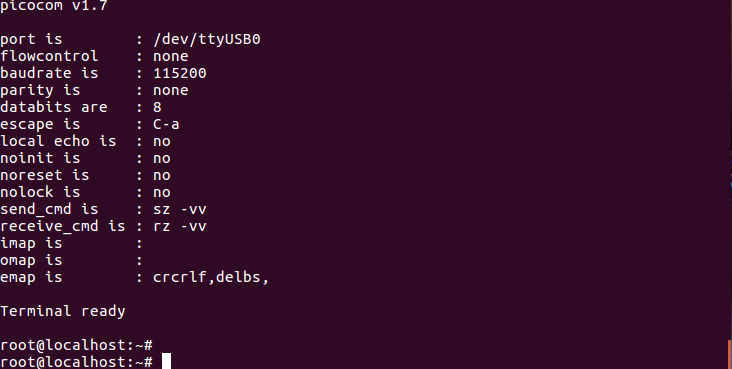
\includegraphics[width=0.7\textwidth]{img/picocom.png}
    \caption{Picocom Terminal Emulator}
    \label{fig:picocom}
\end{figure}


    \item Close the communication by pressing CTRL-A and then CTRL-X

    \item You shall see  \cref{appendix:graph} for other settings and installation process.
\end{enumerate}

{\color{red} \textbf{Optional:}} If you have a screen with an HDMI port, you can connect it to the board (Figure \ref{fig:hdmi}). You can also connect a mouse and a keyboard, but you will need a USB-OTG cable (miniUSB - to - standard USB).



\begin{figure}[h!]
    \centering
    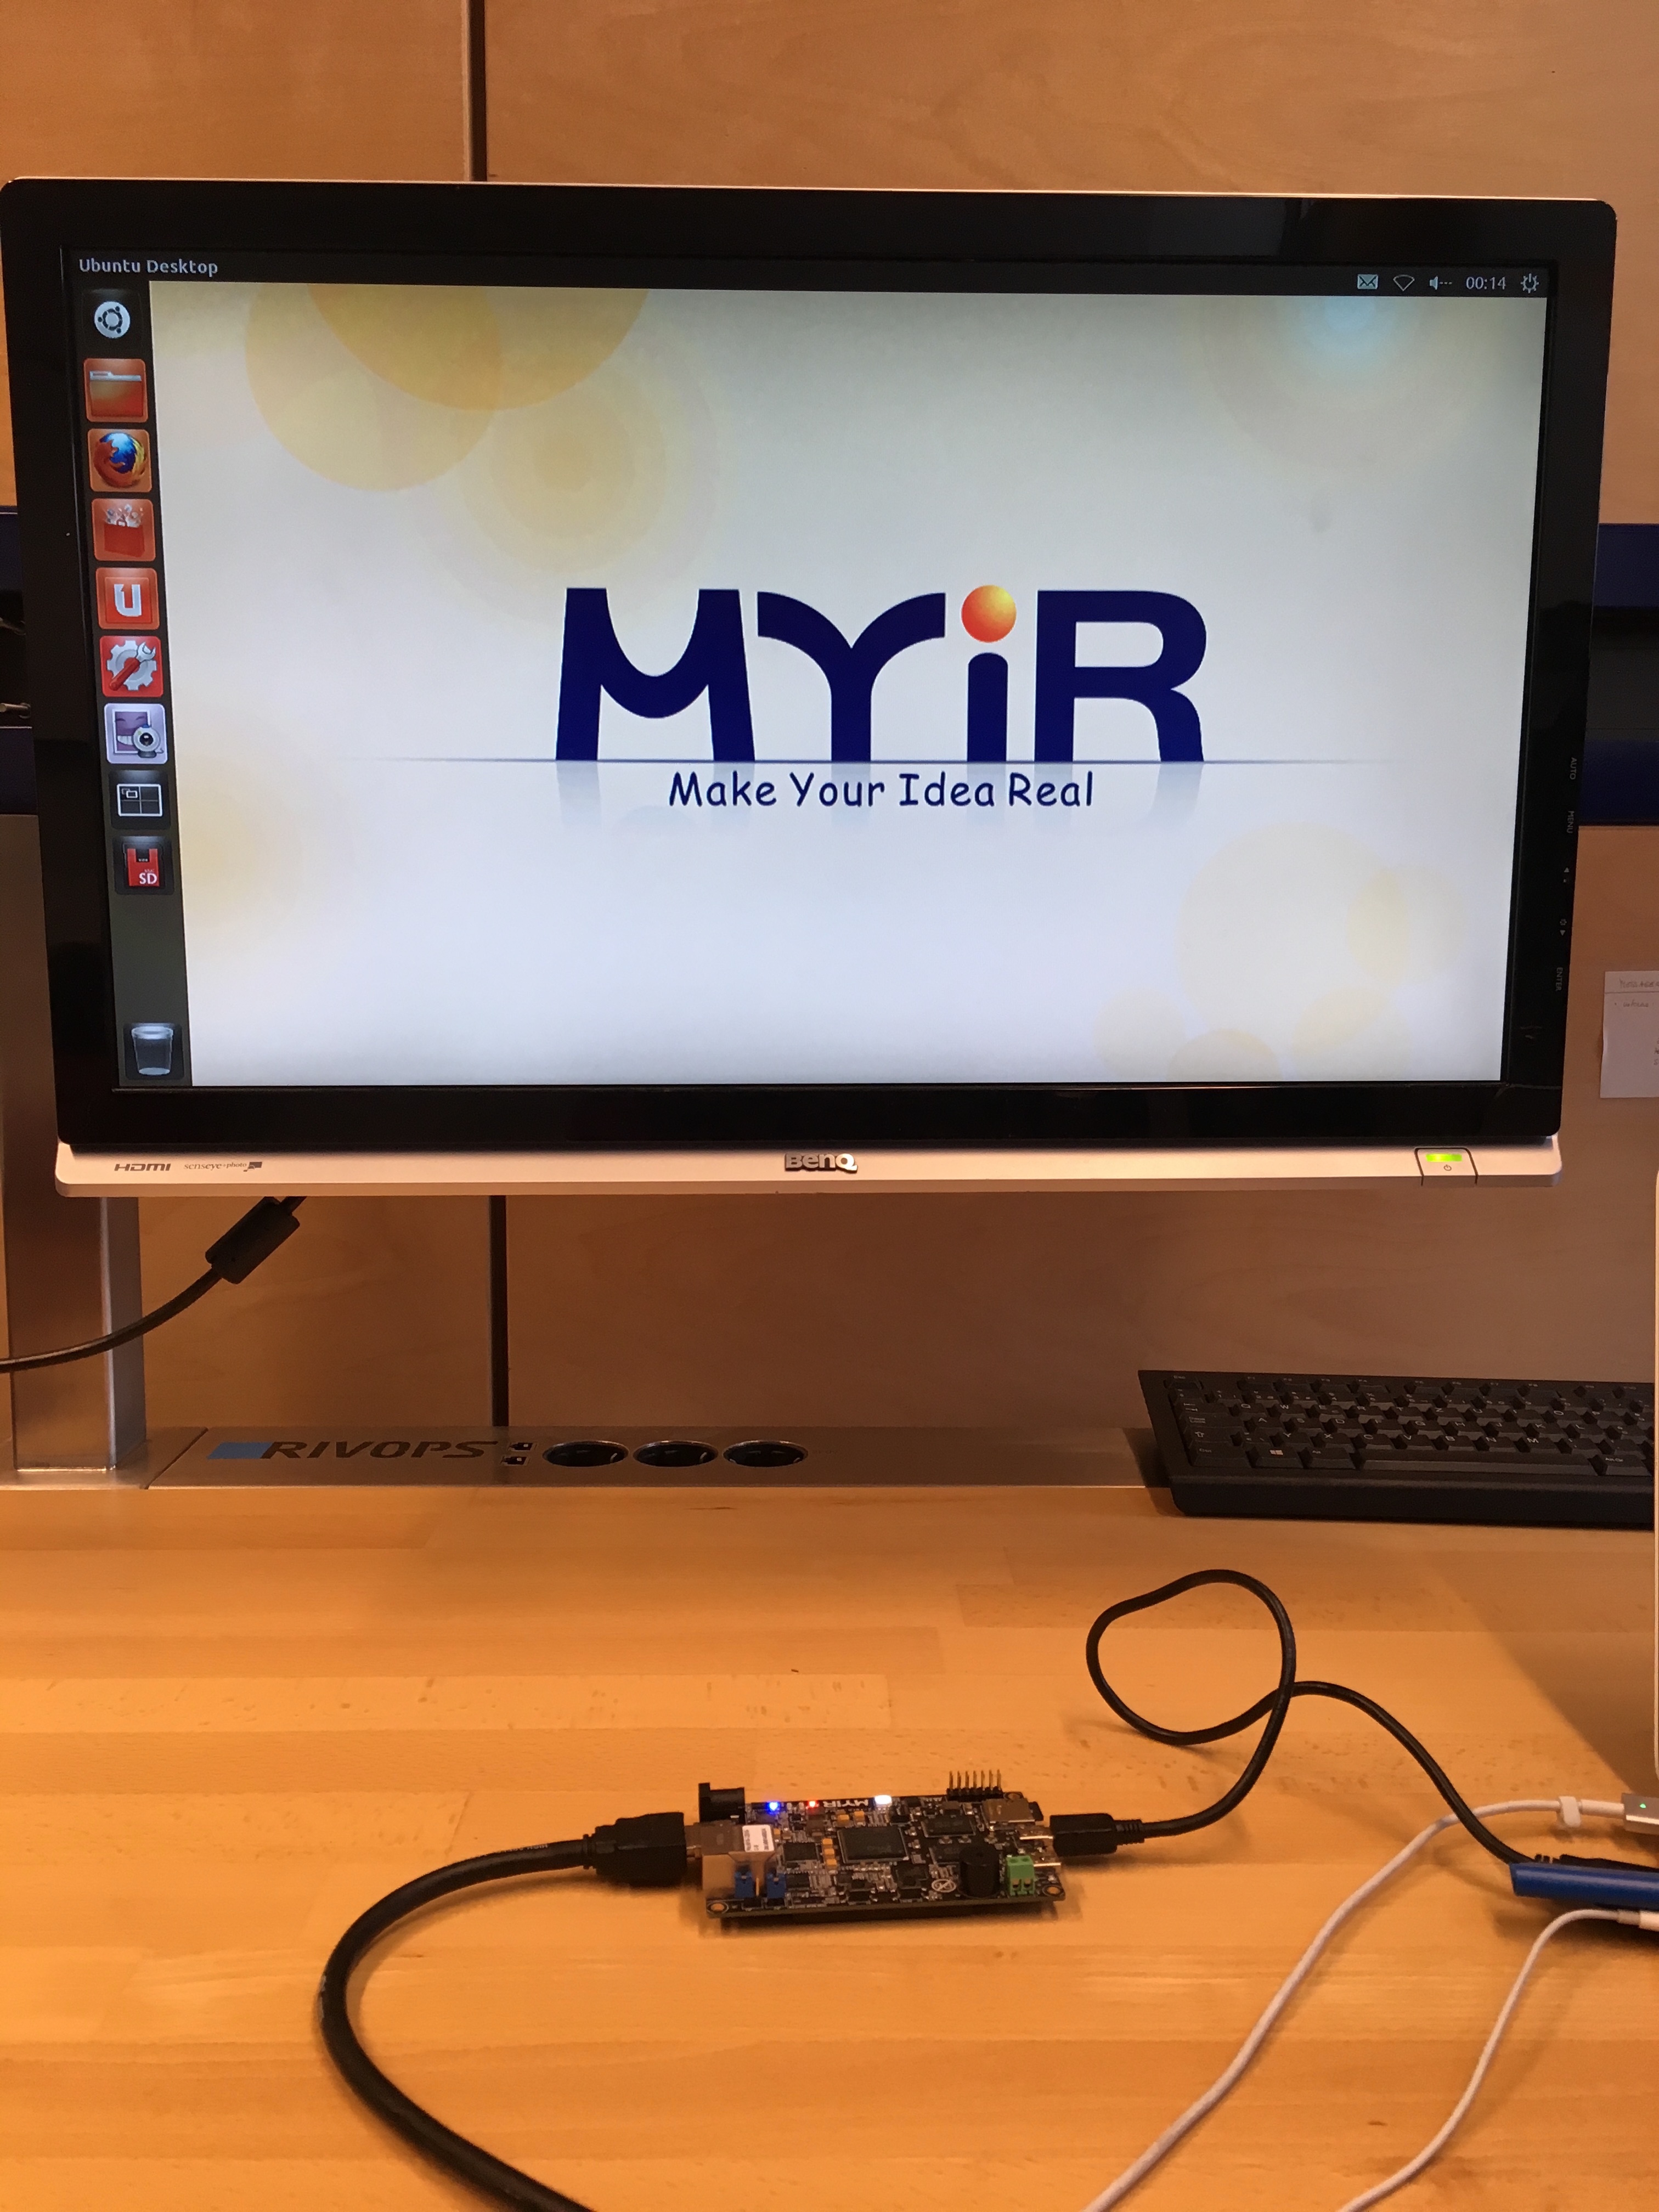
\includegraphics[width=0.6\textwidth]{img/hdmi.JPG}
    \caption{Screen connected to the board}
    \label{fig:hdmi}
\end{figure}


\clearpage
\subsection{Transfer of files between the host computer and the devkit}

In the current lab, we will develop source code on the host computer that needs to be transfered to the board.

There are three methods to transfer files:
\begin{myitemize}
\item Through UART serial protocol
\item Using SCP (Secure CoPy) - a simple transfer tool used to copy one or more files, often with known names, from host A (the computer) to host B (the board) or viceversa
\item Using SFTP (SSH File Transfer Protocol) - which is also a transfer tool used to copy files, but in addition it allows directory listings, remote directories and files removal, creation of files etc.
\end{myitemize}

To simplify life, we will use SCP. Never use UART unless you have a passion to encode/decode data or if other options are not available.

The SSH is already installed on the board. The settings can be seen in \cref{appendix:b}.

The following steps shall be performed: 
\begin{enumerate}
    \item Connect the Ethernet cable between your computer and the board
    \item Type in a new terminal the following command to connect to the board through SSH protocol.
    \begin{tcolorbox}
        \begin{minted}{c}
ssh root@192.168.2.2
        \end{minted}
    \end{tcolorbox}
    You will see basically the same shell as before \ref{fig:picocom}.
    Don't forget that you also need to configure the IP on your computer. For this lab, this work was already done for you.

    \item Next, we will transfer a file to the board.

    On the Desktop, in folder \textit{Laboratory}, you will find a file entitled \textit{lab.py}. This part will contain the final application that you are going to run. Right now, we will just take this file and transfer it to the board, and later on run it.

    For this, \textbf{open a new terminal window} and type the next command in the box. The two points ":" at the end of the next command will place the file in the User folder.
    \begin{tcolorbox}
     \begin{minted}{c}
scp -r ~/Desktop/Laboratory/lab.py root@192.168.2.2:
    \end{minted}
    \end{tcolorbox}






\end{enumerate}




\subsection{Control the LEDs and the buzzer mounted on the devkit}


\begin{enumerate}
\item Make sure you have the emulator opened, by typing:

   \begin{tcolorbox}
        \begin{minted}{c}
ssh root@192.168.2.2
        \end{minted}
    \end{tcolorbox}


\item Control the LEDs

In its simplest form, the LED class just allows control of LEDs from userspace. LEDs appear in $/sys/class/leds/$. Let's check them.

Type in the terminal:
   \begin{tcolorbox}
        \begin{minted}{c}
ls /sys/class/leds/
        \end{minted}
    \end{tcolorbox}

Right now, you shall see the following options:

   \begin{tcolorbox}
        \begin{minted}{c}
led_b  led_g  led_r  mmc0::  usr_led1  usr_led2
        \end{minted}
    \end{tcolorbox}

The first three refer to the RGB LED available on the platform, while the last two refer to LED D29 and D30 on the same board. The LED can be turned on and off using the 'brightness' file. The minimum brightness is 0, and the maximum is 255. As there is no variable brightness support, any value greater than 0 will turn the LED on. Now, let's turn on LED D29 and LED D30. For this, you need to type in the emulator:

   \begin{tcolorbox}
        \begin{minted}{c}
echo 1 > /sys/class/leds/usr_led1/brightness
echo 1 > /sys/class/leds/usr_led2/brightness
        \end{minted}
    \end{tcolorbox}

Check the result on the board.

{\textbf{\color{red}Optional:}} Implement your own toggle (on and off) of the RGB LED in a python script. In case you get stuck, check the Appendix \cref{appendix:E}.



\item Control the BUZZER

The buzzer is seen as a device. "In Unix-like operating systems, a device file or special file is an interface for a device driver that appears in a file system as if it were an ordinary file.They allow software to interact with a device driver using standard input/output system calls, which simplifies many tasks and unifies user-space I/O mechanisms. "(Source: Wikipedia). They can be found in $/dev/input/eventX$. Let's see them by typing:

   \begin{tcolorbox}
        \begin{minted}{c}
ls /dev/input/
        \end{minted}
    \end{tcolorbox}

You can thus see, a list of events. But how do we know which one is applicable to the Buzzer?

Let's write a Python script to access them. We will use the python-evdev library which allows you to read and write input events on Linux.

Open a new file, call it "buzzer.py" and write the following lines of code to get information for event0, event1 and event2

   \begin{tcolorbox}
        \begin{minted}{python}
from evdev import InputDevice, ecodes
import time

device0 = InputDevice('/dev/input/event0')
device1 = InputDevice('/dev/input/event1')
device2 = InputDevice('/dev/input/event2')

print(device0)
print(device1)
print(device2)
        \end{minted}
    \end{tcolorbox}


You can  see that the first two are actually the buzzer device and the accelerometer device, the ones that we need to use.

Let's turn the buzzer ON. For this, you need to add the following lines of code to the previous ones:

   \begin{tcolorbox}
        \begin{minted}{python}
device0.write(ecodes.EV_SND, ecodes.SND_BELL, 1)
time.sleep(2)
device0.write(ecodes.EV_SND, ecodes.SND_BELL, 0)
print(device0.capabilities(verbose=True))
        \end{minted}
    \end{tcolorbox}


We understood how InputDevice works, but, what are \textbf{ecodes} and why they are used in the previous lines of code to access the buzzer?

An input event is represented by standard $input\_event$ structure defined in $linux/input.h$ header file. According to this header file,  the structure is: 
\begin{myitemize}
\item timestamp
\item type $->$ EV\_SND (for the buzzer)
\item code $->$ SND\_BELL (for the buzzer)
\item value $->$ (1 or 0 for ON and OFF)
\end{myitemize}


\end{enumerate}



\subsection{Read accelerometer data}

In the previous part, we saw that the accelerometer can be accessed from $/dev/input/event1$. 


\noindent\rule{16.5cm}{1pt}

\noindent\begin{minipage}{.1\textwidth}
  \centering
  
\includegraphics[height=1.5cm]{img/icon.png}
\end{minipage}
\begin{minipage}{.8\textwidth}
Now it's your turn to read the device and display the accelerometer data. To understand how to do this, you need to read the documentation of python-evdev library. 
\url{http://python-evdev.readthedocs.io/en/latest/}. If you get stuck, check Appendix \cref{appendix:D}.
\end{minipage}%

\noindent\rule{16.5cm}{1pt}



\subsection{Webserver}
Now, we will see how to display the accelerometer values on an webserver running on the host computer.

For this part, Bokeh was used. Bokeh is a Python interactive visualization library that targets modern web browsers for presentation. Its goal is to provide elegant, concise construction of novel graphics.

To run the webserver, you need to type in the emulator the following:

   \begin{tcolorbox}
        \begin{minted}{c}
bokeh serve --host 192.168.2.2:5006 read_event.py
        \end{minted}
    \end{tcolorbox}


Then, in your host computer, open a webbrowser and type the IP, as seen in Figure \ref{fig:bokeh}.

\begin{figure}[h!]
    \centering
    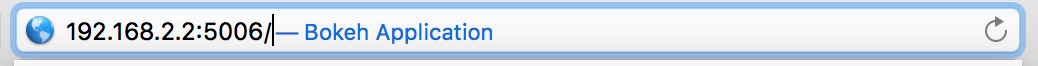
\includegraphics[width=0.6\textwidth]{img/bokeh.png}
    \caption{Host address}
    \label{fig:bokeh}
\end{figure}

Then, the plot will be displayed interactively! Have fun!

\begin{figure}[h!]
    \centering
    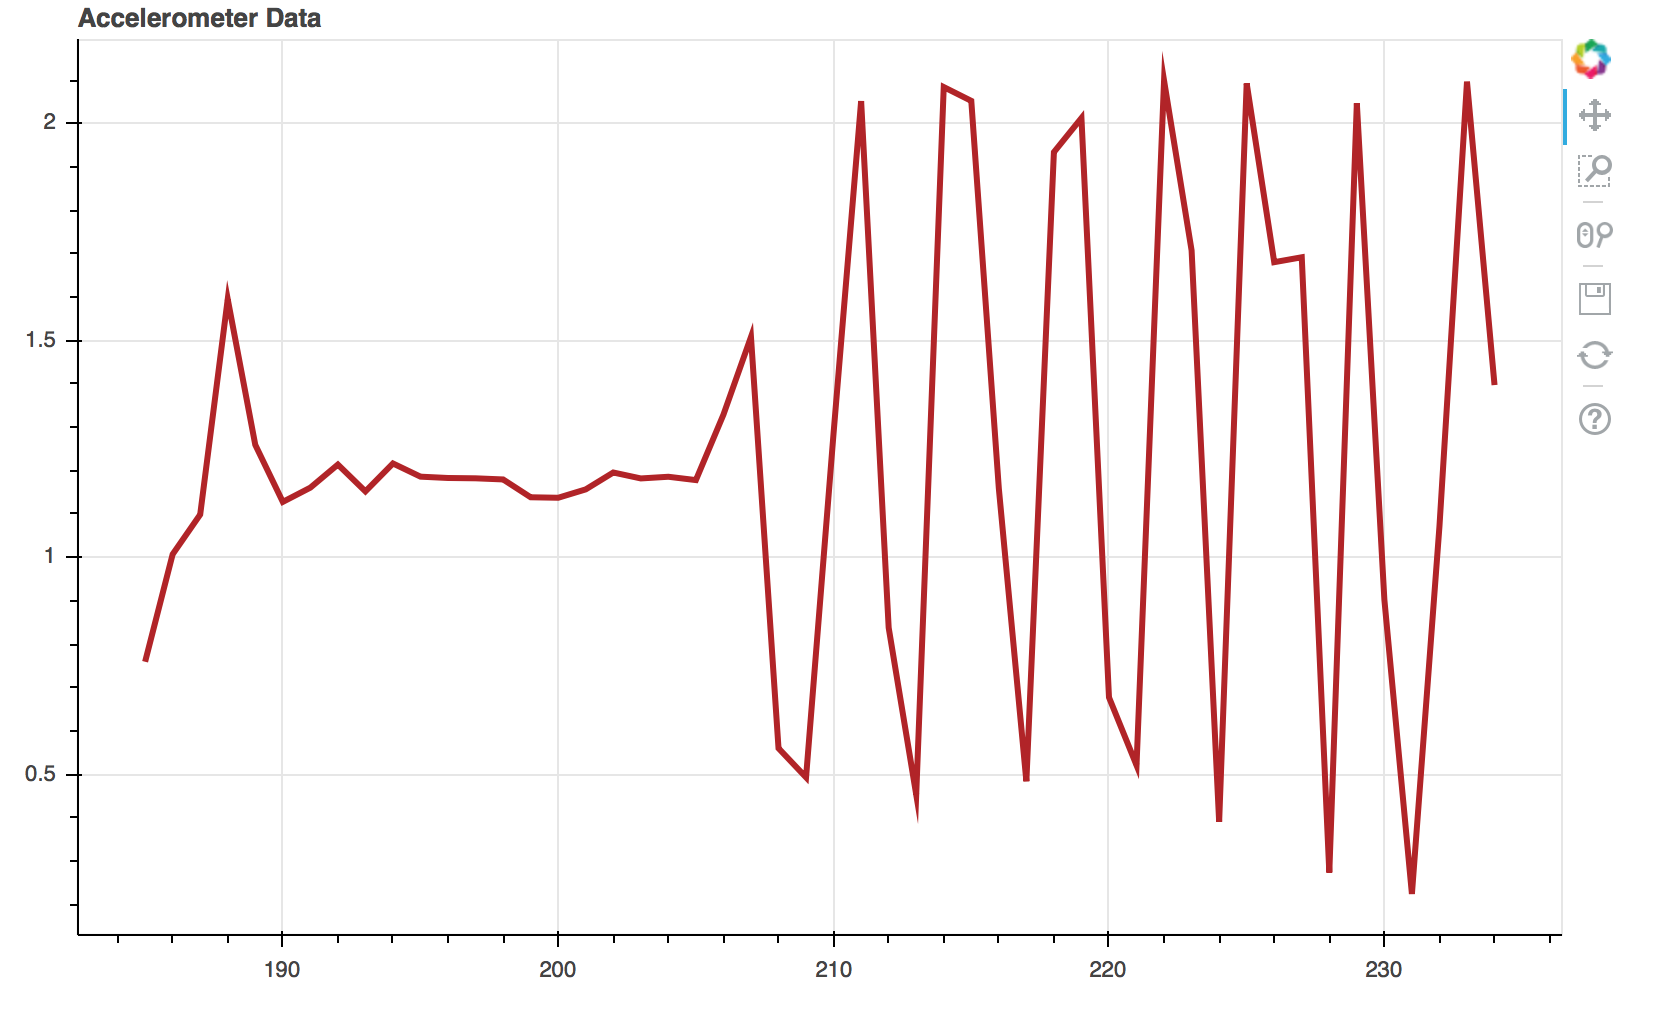
\includegraphics[width=0.6\textwidth]{img/acc.png}
    \caption{Host address}
    \label{fig:bokeh}
\end{figure}



